\documentclass[notes,11pt, aspectratio=169]{beamer}

\usepackage{pgfpages}
% These slides also contain speaker notes. You can print just the slides,
% just the notes, or both, depending on the setting below. Comment out the want
% you want.
\setbeameroption{hide notes} % Only slide
%\setbeameroption{show only notes} % Only notes
%\setbeameroption{show notes on second screen=right} % Both

\usepackage{helvet}
\usepackage[default]{lato}
\usepackage{array}
\usepackage{tgbonum}

\usepackage{tikz}
\usepackage{verbatim}
\setbeamertemplate{note page}{\pagecolor{yellow!5}\insertnote}
\usetikzlibrary{positioning}
\usetikzlibrary{snakes}
\usetikzlibrary{calc}
\usetikzlibrary{arrows}
\usetikzlibrary{decorations.markings}
\usetikzlibrary{shapes.misc}
\usetikzlibrary{matrix,shapes,arrows,fit,tikzmark}
\usepackage{amsmath}
\usepackage{mathpazo}
\usepackage{hyperref}
\usepackage{lipsum}
\usepackage{multimedia}
\usepackage{graphicx}
\usepackage{multirow}
\usepackage{graphicx}
\usepackage{dcolumn}
\usepackage{bbm}
\newcolumntype{d}[0]{D{.}{.}{5}}

\usepackage{changepage}
\usepackage{appendixnumberbeamer}
\newcommand{\beginbackup}{
   \newcounter{framenumbervorappendix}
   \setcounter{framenumbervorappendix}{\value{framenumber}}
   \setbeamertemplate{footline}
   {
     \leavevmode%
     \hline
     box{%
       \begin{beamercolorbox}[wd=\paperwidth,ht=2.25ex,dp=1ex,right]{footlinecolor}%
%         \insertframenumber  \hspace*{2ex} 
       \end{beamercolorbox}}%
     \vskip0pt%
   }
 }
\newcommand{\backupend}{
   \addtocounter{framenumbervorappendix}{-\value{framenumber}}
   \addtocounter{framenumber}{\value{framenumbervorappendix}} 
}


\usepackage{graphicx}
\usepackage[space]{grffile}
\usepackage{booktabs}
\newcommand\independent{\protect\mathpalette{\protect\independenT}{\perp}}
\def\independenT#1#2{\mathrel{\rlap{$#1#2$}\mkern2mu{#1#2}}}
\DeclareMathOperator{\Supp}{Supp}

% These are my colors -- there are many like them, but these ones are mine.
\definecolor{blue}{RGB}{0,114,178}
\definecolor{red}{RGB}{213,94,0}
\definecolor{yellow}{RGB}{240,228,66}
\definecolor{green}{RGB}{0,158,115}

\hypersetup{
  colorlinks=false,
  linkbordercolor = {white},
  linkcolor = {blue}
}


%% I use a beige off white for my background
\definecolor{MyBackground}{RGB}{255,253,218}

%% Uncomment this if you want to change the background color to something else
%\setbeamercolor{background canvas}{bg=MyBackground}

%% Change the bg color to adjust your transition slide background color!
\newenvironment{transitionframe}{
  \setbeamercolor{background canvas}{bg=yellow}
  \begin{frame}}{
    \end{frame}
}

\setbeamercolor{frametitle}{fg=blue}
\setbeamercolor{title}{fg=black}
\setbeamertemplate{footline}[frame number]
\setbeamertemplate{navigation symbols}{} 
\setbeamertemplate{itemize items}{-}
\setbeamercolor{itemize item}{fg=blue}
\setbeamercolor{itemize subitem}{fg=blue}
\setbeamercolor{enumerate item}{fg=blue}
\setbeamercolor{enumerate subitem}{fg=blue}
\setbeamercolor{button}{bg=MyBackground,fg=blue,}



% If you like road maps, rather than having clutter at the top, have a roadmap show up at the end of each section 
% (and after your introduction)
% Uncomment this is if you want the roadmap!
% \AtBeginSection[]
% {
%    \begin{frame}
%        \frametitle{Roadmap of Talk}
%        \tableofcontents[currentsection]
%    \end{frame}
% }
\setbeamercolor{section in toc}{fg=blue}
\setbeamercolor{subsection in toc}{fg=red}
\setbeamersize{text margin left=1em,text margin right=1em} 

\newenvironment{wideitemize}{\itemize\addtolength{\itemsep}{10pt}}{\enditemize}

\usepackage{environ}
\NewEnviron{videoframe}[1]{
  \begin{frame}
    \vspace{-8pt}
    \begin{columns}[onlytextwidth, T] % align columns
      \begin{column}{.70\textwidth}
        \begin{minipage}[t][\textheight][t]
          {\dimexpr\textwidth}
          \vspace{8pt}
          \hspace{4pt} {\Large \sc \textcolor{blue}{#1}}
          \vspace{8pt}
          
          \BODY
        \end{minipage}
      \end{column}%
      \hfill%
      \begin{column}{.38\textwidth}
        \colorbox{green!20}{\begin{minipage}[t][1.2\textheight][t]
            {\dimexpr\textwidth}
            Face goes here
          \end{minipage}}
      \end{column}%
    \end{columns}
  \end{frame}
}

\title[]{\textcolor{blue}{Research Design, Randomization and Design-Based Inference }}
\author[PGP]{}
\institute[FRBNY]{\small{Paul Goldsmith-Pinkham}}
\date{\today}


\begin{document}

%%% TIKZ STUFF
\tikzset{   
        every picture/.style={remember picture,baseline},
        every node/.style={anchor=base,align=center,outer sep=1.5pt},
        every path/.style={thick},
        }
\newcommand\marktopleft[1]{%
    \tikz[overlay,remember picture] 
        \node (marker-#1-a) at (-.3em,.3em) {};%
}
\newcommand\markbottomright[2]{%
    \tikz[overlay,remember picture] 
        \node (marker-#1-b) at (0em,0em) {};%
}
\tikzstyle{every picture}+=[remember picture] 
\tikzstyle{mybox} =[draw=black, very thick, rectangle, inner sep=10pt, inner ysep=20pt]
\tikzstyle{fancytitle} =[draw=black,fill=red, text=white]
%%%% END TIKZ STUFF

% Title Slide
\begin{frame}
\maketitle

\end{frame}

\begin{frame}{Outline on Randomization}
  \begin{wideitemize}
    \item Discuss the value of randomized interventions, and identifying settings where interventions are ``as-if'' randomly assigned
   \begin{itemize}
     \item Touch on the historical and (somewhat) current views on this
    \end{itemize}
  \item Define a ``research design.''
  \item Give an introduction to design-based vs. model-based identification and causal inference.
\end{wideitemize}
\end{frame}


% INTRO
\begin{frame}{The power of randomization}
\begin{columns}[T] % align columns
\begin{column}{.65\textwidth}
  \begin{wideitemize}
  \item Randomization is a powerful tool
    \begin{itemize}
    \item E.g. An intervention giving a treatment to half of a sample
      using a randomized process
    \item Formally, randomly assign $D_{i}$ to a sample of size
      $n$ such that the set of potential random assignments across all
      $n$ individuals is known ($\Omega$), and the probability
      distribution over $\Omega$ is known
    \item In other words, you know the ``true'' propensity to receive treatment (the p-score)
    \end{itemize}
  \item In our different models of causal inference:
    \begin{itemize}
    \item<2-> randomized intervention breaks paths on DAG      
    \item<4-> Creates independence necessary for strong ignorability
    \item<5-> Creates \emph{some} forms of independence between the
      intervention and structural errors in a model
      \begin{itemize}
      \item Why only some?
      \end{itemize}
    \end{itemize}
  \end{wideitemize}
\end{column}%
\hfill%
\begin{column}{.4\textwidth}
  \begin{center}
    \only<2>{
      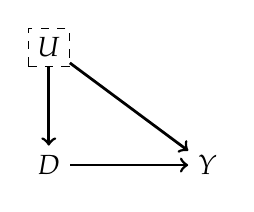
\begin{tikzpicture}
        % nodes %
        % \node[text centered] (z) {$Z$};
        \node[text centered] (t) {$D$};
        \node[right=1.5 of t, text centered] (y) {$Y$};
        \node[draw, rectangle, dashed, above = 1 of t, text centered] (u) {$U$};

        % edges %
        % \draw[->, line width= 1] (z) --  (t);
        \draw [->, line width= 1] (t) -- (y);
        % \draw[->,red, line width= 1,dashed] (u) --node {X} (z);
        \draw[->,line width= 1] (u) --(t);
        \draw[->,line width= 1] (u) -- (y);
%\draw[->, red, line width=1,dashed] (z) to  [out=270,in=270, looseness=0.5] node{X} (y);
      \end{tikzpicture}
      }
    \only<3>{
      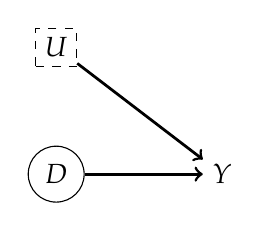
\begin{tikzpicture}
        % nodes %
        % \node[text centered] (z) {$Z$};
        \node[draw, circle, text centered] (t) {$D$};
        \node[right=1.5 of t, text centered] (y) {$Y$};
        \node[draw, rectangle, dashed, above = 1 of t, text centered] (u) {$U$};

        % edges %
        % \draw[->, line width= 1] (z) --  (t);
        \draw [->, line width= 1] (t) -- (y);
        % \draw[->,red, line width= 1,dashed] (u) --node {X} (z);
        %\draw[->,line width= 1] (u) --(t);
        \draw[->,line width= 1] (u) -- (y);
%\draw[->, red, line width=1,dashed] (z) to  [out=270,in=270, looseness=0.5] node{X} (y);
      \end{tikzpicture}
    }
    \only<5>{
      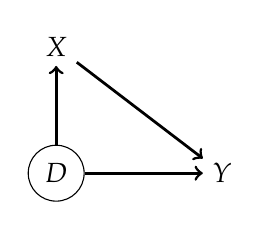
\begin{tikzpicture}
        % nodes %
        % \node[text centered] (z) {$Z$};
        \node[draw, circle, text centered] (t) {$D$};
        \node[right=1.5 of t, text centered] (y) {$Y$};
        \node[above = 1 of t, text centered] (x) {$X$};

        % edges %
        % \draw[->, line width= 1] (z) --  (t);
        \draw [->, line width= 1] (t) -- (y);
        % \draw[->,red, line width= 1,dashed] (u) --node {X} (z);
        %\draw[->,line width= 1] (u) --(t);
        \draw[->,line width= 1] (t) -- (x);
        \draw[->,line width= 1] (x) -- (y);        
%\draw[->, red, line width=1,dashed] (z) to  [out=270,in=270, looseness=0.5] node{X} (y);
      \end{tikzpicture}
      \begin{itemize}
      \item Imagine an intervention that affects multiple outcomes
      \item Even randomized, if agents reoptimize with respect to $X$,
        this intervention no longer identifies the exclusive effect of $D$ on $Y$ without more assumptions
      \end{itemize}
      }
    \end{center}

\end{column}%
\end{columns}
\end{frame}

\begin{frame}{If the use of randomization is so powerful, why don't we always use it?}
  There are a few reasons:
  \begin{enumerate}
    \item People may not want to be randomized into different treatments. 
    \begin{itemize}
      \item They value their choices, and it may be impractical to randomize their decisions even if there is a clear benefit to doing so. 
      \item A firm, for example, may not want to randomize their policies
    \end{itemize}
    \item It may be unethical to randomize.
    \begin{itemize}
      \item For example, if there is a clear benefit to a treatment, it may be unethical to withhold that treatment from individuals by placing them in the control.
    \end{itemize}
    \item It may be impossible to randomize. 
    \begin{itemize}
      \item For example, if we are interested in the effect of a policy change, it may be impossible to randomize the policy change across different regions or states.
    \end{itemize}
  \end{enumerate}
\end{frame}

\begin{frame}{A historical aside on the credibility revolution}
\begin{columns}[T] % align columns
  \begin{column}{.4\textwidth}
    \begin{itemize}
    \item A director's cut of ``Let's take the con out of econometrics'' Leamer (1983)
    \end{itemize}
\end{column}%
\hfill%
\begin{column}{.6\textwidth}
  \vspace{-8pt}
  \begin{center}
  \only<2>{\includegraphics[width=0.7\linewidth]{images/leamer1.png}}
  \only<3>{\includegraphics[width=0.6\linewidth]{images/leamer2.png}}
  \only<4>{\includegraphics[width=0.7\linewidth]{images/leamer3.png}}
  \only<5>{\includegraphics[width=0.7\linewidth]{images/leamer4.png}}
  \only<6>{
    \includegraphics[width=0.6\linewidth]{images/leamer5.png}\\
    \includegraphics[width=0.55\linewidth]{images/leamer5b.png}}
  \only<1>{
    \includegraphics[width=0.7\linewidth]{images/leamer6a.png}\\
    \includegraphics[width=0.7\linewidth]{images/leamer6b.png}\\    
  }  
  \end{center}
\end{column}%
\end{columns}
\end{frame}

\begin{frame}{A historical aside on the credibility revolution}
\begin{columns}[T] % align columns
  \begin{column}{.4\textwidth}
    \begin{wideitemize}
    \item Important context for understanding current empirical
      methodology: empirics was viewed with tremendous skepticism by the 1980s
    \item Here's Black (1982)
    \end{wideitemize}
\end{column}%
\hfill%
\begin{column}{.6\textwidth}
    \includegraphics[width=0.9\linewidth]{images/black1.png}\\
\end{column}%
\end{columns}
\end{frame}

\begin{frame}{A historical aside on the credibility revolution}
\begin{columns}[T] % align columns
  \begin{column}{.4\textwidth}
    \begin{wideitemize}
    \item Fast-forward 25 years later and Angrist and Pischke (2010) have declared a credibility revolution
    \item ``Reseach design'' is the clear victor, with pure randomization the leading champion
    \end{wideitemize}
\end{column}%
\hfill%
\begin{column}{.6\textwidth}
  \includegraphics[width=0.9\linewidth]{images/angristpishke2010.png}\\
  \includegraphics[width=0.9\linewidth]{images/angristpishke2010b.png}\\
\end{column}%
\end{columns}
\end{frame}

\begin{frame}{What is a research design?}
\begin{columns}[T] % align columns
  \begin{column}{.7\textwidth}
    \begin{wideitemize}
    \item A clear interpretation from this is that ``research design''
      is important.
    \item Well, what's the right definition for research design?
      \begin{itemize}
      \item Shows up 69 times in Angrist and Pischke's JEP piece, but not defined 
      \end{itemize}
    \item It seems almost ``intuitive'' but let's try to define it.
    \end{wideitemize}
\end{column}%
\hfill%
\begin{column}{.6\textwidth}
\end{column}%
\end{columns}
\end{frame}

\begin{frame}{David Card's definition of Research Design}
  \begin{wideitemize}
  \item Card draws a distinction between causality as ``model-based'' and ``design-based'':
    \begin{itemize}
    \item ``causality is model-based: only exists within the framework of a theory that x causes y''
    \item ``causality is design-based: ...causality requires that you can design a manipulation in which x causes y''
    \end{itemize}
  \item Crucial definition of what Card views as ``design-based'' approach:
    \begin{itemize}
    \item ``identification equated with research design''
    \item ``research design defines the counterfactual''
    \item Of course, he also doesn't define (in his slides) what research design means...
    \end{itemize}
  \item From Card's Nobel lecture: research design is equated with
    transparently describibng sources of identification
    \item   \url{https://davidcard.berkeley.edu/lectures/woytinsky.pdf}
  \end{wideitemize}
\end{frame}

\begin{frame}{Paul Goldsmith-Pinkham's definition of Research Design}
\begin{columns}[T] % align columns
  \begin{column}{\textwidth}
    \begin{wideitemize}
    \item A \emph{(causal) research design} is a statistical and/or economic
      statement of how an empirical research paper will estimate a
      relationship between two (or more) variables that is causal in nature: how $X$ causes $Y$.

    \item Since we know that causal effects require estimation of an
      (unobservable) counterfactual, a research design describes what
      assumptions are necessary to estimate the counterfactual(s) for a
      given estimand.
      
    \item As we will discuss in class, these research designs can be
      split into two types of assumptions (with some overlap to be
      discussed later):
      \begin{itemize}
      \item \emph{Model}-based: the estimand is
        identified using assumptions on the modeling of the potential outcomes conditional on treatment and additional variables
         (e.g. parallel trends)
       \item\emph{Design}-based: the estimand is
         identified using assumptions on the treatment variable,
         conditional on the potential outcomes and additional
         variables
      \end{itemize}

      \item They are different \emph{assumptions} to allow for credible estimates
    \end{wideitemize}
\end{column}%
\hfill%
\begin{column}{.6\textwidth}
\end{column}%
\end{columns}
\end{frame}


\begin{frame}{Why was research design revolution so important?}
\begin{columns}[T] % align columns
  \begin{column}{.7\textwidth}
    \begin{wideitemize}
    \item For today, we'll assume we have a randomized intervention: an example of a design-based approach
      \begin{itemize}
      \item Ignore compliance
      \item Ignore ``quasi-experimental'' vagaries
      \item These are all solveable! See Bowers and Leavitt (2020) for discussion
      \end{itemize}
    \item Knowledge of an explicit, randomized design provides a different
      approach to estimation and testing than what we traditionally learn in econometrics
    \item \emph{Design-based} inference is
      \begin{enumerate}
      \item Transparent
      \item Efficient
      \end{enumerate}
    \item Today: basic primer to give groundwork for rest of course
      \begin{itemize}
      \item Very useful in some situations!
      \end{itemize}
    \end{wideitemize}
\end{column}%
\hfill%
\begin{column}{.6\textwidth}
\end{column}%
\end{columns}
\end{frame}

\begin{frame}{What is goal of design-based inference?}
  \begin{wideitemize}
  \item Potential outcomes framework highlights that we can talk about every unit's PO.
    \begin{itemize}
    \item Let there be a \emph{finite} population of $n$ individuals,
      $i = \{1, \ldots, n\}$
    \item For each $i$, we have $(Y_{i}(0), Y_{i}(1), D_{i})$, where
      $(Y_{i}(0), Y_{i}(1))$ denote their set of potential outcomes,
      and $D_{i} \in \{0,1\}$ denote their treatment status
    \item Let $\mathbf{Y}_{0}$ denote the vector of $Y_{i}(0)$,
      $\mathbf{Y}_{1}$ denote the vector of $Y_{i}(1)$, and
      $\mathbf{D}_{0}$ denote the vector of $D_{i}$.
    \end{itemize}
  \item What do we want to know / test about these outcomes?
    \begin{itemize}
    \item Average? Distribution? Shifts? Underlying parameter?
    \item For now, we'll focus on additive difference
      $\tau_{i} = Y_{i}(1) - Y_{i}(0)$, and the average of it
      $\bar{\tau} = n^{-1}\sum_{i=1}^{n}\tau_{i}.$
    \end{itemize}
  \item What do we want to do?
    \begin{itemize}
    \item Let's start by making $\bar{\tau}$ our \emph{estimand}
    \end{itemize}
  \end{wideitemize}
\end{frame}

\begin{frame}{Define our research design}
\begin{columns}[T] % align columns
  \begin{column}{.7\textwidth}
  \begin{wideitemize}
  \item Consider the set of potential ways that $\mathbf{D}$ could be randomized to the population
    \begin{itemize}
    \item $\mathbf{Y}_{1}$ and $\mathbf{Y}_0$ are \emph{fixed} -- it
      is only the random variation in $\mathbf{D}$ that creates
      uncertainty
    \end{itemize}
  \item Let $\Omega$ denote that space of possible values that
      $\mathbf{D}$ can take. It is defined by the type of randomize
      experiment one runs.
      \begin{itemize}
      \item If we do a purely randomized individualized trial, where
        each individual has a fair coin flipped on whether they are
        treatment or control, then $\Omega = \{0,1\}^{n}$. But then
        the variation in number treated and control can vary quite a
        lot for small samples!
      \item Other ways to consider randomly assigning individuals
        \begin{itemize}
        \item Random draws from an urn (to ensure an exact number treated)
        \item Clustering individuals on characteristics (or location)
        \end{itemize}
      \end{itemize}
    \end{wideitemize}
  \end{column}%
  \hfill%
  \begin{column}{.4\textwidth}
    \includegraphics[width=\linewidth]{images/randomized1.pdf}
  \end{column}%
\end{columns}
\end{frame}

\begin{frame}{Define our research design}
\begin{columns}[T] % align columns
  \begin{column}{.7\textwidth}
  \begin{wideitemize}
  \item Key point: we know the exact probability distribution over
    $\Omega$, and hence $\mathbf{D}$.
  \item<2-> First consider with full knowledge for the true draw of
    $\mathbf{D}$ (the assignment that happened in our data)
  \item<3-> The fundamental problem of causal inference  binds
    \begin{itemize}
    \item Now, if we enforce that 50\% is always treated, we know that
      there are only ${10 \choose 5}= 252$ potential combinations
      (each equally likely).
    \end{itemize}

    \end{wideitemize}
  \end{column}%
  \hfill%
  \begin{column}{.4\textwidth}
    \only<2>{
    \begin{tabular}{cccc}
      \toprule
      $D_{i}$ & $Y_{i}(1)$ & $Y_{i}(0)$ & $Y_{i}$\\
      \midrule
      1 &  11.9 &  6.6 & 11.9\\
      1 &  10   &  8.5 & 10\\
      1 &  9.7  &  9.4 & 9.7\\
      1 &  9.5  &   7 & 9.5 \\
      1 &  11.4 &  7.4 & 11.4\\
      0 &  9.6 &  7.6 & 7.6\\
      0 &  9.1  & 7.1  & 7.1\\
      0 &  10.4 &  7.7  & 7.7\\
      0 &  10.4 &  8 & 8  \\
      0 & 12.4  & 7.8 & 7.8\\
      \bottomrule
    \end{tabular}
  }
      \only<3>{
    \begin{tabular}{cccc}
      \toprule
      $D_{i}$ & $Y_{i}(1)$ & $Y_{i}(0)$ & $Y_{i}$\\
      \midrule
      1 &  11.9 &   & 11.9\\
      1 &  10   &   & 10\\
      1 &  9.7  &   & 9.7\\
      1 &  9.5  &  & 9.5 \\
      1 &  11.4 &   & 11.4\\
      0 &   &  7.6 & 7.6\\
      0 &    & 7.1  & 7.1\\
      0 &   &  7.7  & 7.7\\
      0 &   &  8 & 8  \\
      0 &   & 7.8 & 7.8\\
      \bottomrule
    \end{tabular}
    }

  \end{column}%
\end{columns}
\end{frame}

\begin{frame}{Return to our estimand of interest, $\bar{\tau}$}
  \begin{wideitemize}
  \item We now need an estimator for $\bar{\tau} = n^{-1}\sum_{i=1}^{n}\tau_{i}$
  \item We already know under random assignment that $E(Y_{i}| D_{i} = 1) - E(Y_{i} | D_{i} = 0)$ identifies $E(\tau_{i})$
    \begin{itemize}
    \item Take the empirical estimator of this expression:
      $\hat{\bar{\tau}}(\mathbf{D}, \mathbf{Y}) =
      \frac{\mathbf{D}'\mathbf{Y}}{\sum_{i}D_{i}} -
      \frac{(\mathbf{1}-\mathbf{D})'\mathbf{Y}}{\sum_{i}(1-D_{i})}$
    \item Note that this expectation operator is well-defined from the
      objects we already know -- only $D$ is random, and we know its
      marginal distribution over the sample
    \item Can show that under certain assumptions (random assignment
      is equal across $\Omega$) that this estimator is unbiased.
      \begin{itemize}
      \item We can also now construct tests for this estimator that
        are more efficient than model based versions in small samples
      \end{itemize}
    \end{itemize}
  \end{wideitemize}
\end{frame}

\begin{frame}
  
  \begin{wideitemize}
  \item Is it an unbiased estimator in this case?
  \item If we assume that assignment is completely equal, then let
    $\pi_{1}(\mathbf{D}) = n_{t}(\mathbf{D})/n$ be the share treated,
    and $E(\pi_{1}^{-1}D_{i}) = 1$.
    \item Then,
      \begin{align}
        E(\hat{\bar{\tau}}(\mathbf{D}, \mathbf{Y})) &= E\left(\frac{\mathbf{D}'\mathbf{Y}}{\sum_{i}D_{i}} - \frac{(\mathbf{1}-\mathbf{D})'\mathbf{Y}}{\sum_{i}(1-D_{i})}\right)\\
                                                    &=n^{-1}E\left(\sum_{i}\pi_{1}^{-1}Y_{i}D_{i} - \sum_{i}(1-\pi_{1})^{-1}Y_{i}(1-D_{i})\right)\\
                                                    &=n^{-1}E\left(\sum_{i}\pi_{1}^{-1}Y_{i}(1)D_{i} - \sum_{i}(1-\pi_{1})^{-1}Y_{i}(0)(1-D_{i})\right)\\
                                                    &=n^{-1}\sum_{i}Y_{i}(1)E\left(\pi_{1}^{-1}D_{i}\right) - n^{-1}\sum_{i}Y_{i}(0)E\left((1-\pi_{1})^{-1}(1-D_{i})\right)\\
        &=n^{-1}\sum_{i}Y_{i}(1) - Y_{i}(0) = n^{-1}\sum_{i}\tau_{i}
        %\sum_{\mathbf{d} \in \Omega} n^{-1}_{t}(\mathbf{d})\sum_{i} Y_{i}\times Pr(\mathbf{D} = \mathbf{d})
      \end{align}
    \end{wideitemize}
\end{frame}


\begin{frame}{Variance of $\hat{\tau}$}
  \begin{wideitemize}
  \item The variance of $\hat{\tau}$ (based on the sampling variation
    in the random design) is known thanks to Neyman (1923)
    \begin{equation}
      \sigma^{2}_{\hat{\bar{\tau}}} = \frac{1}{n-1}\left(\frac{n_{t}\sigma^{2}_{0}}{n_{c}} + \frac{n_{c} \sigma^{2}_{1}}{n_{t}} + 2\sigma_{0,1}\right)
    \end{equation}
    where $n_{t}$ and $n_{c}$ are the number of treated and control
    individuals ($n_{t} + n_{c} = n$) and
    $\sigma^{2}_{0}, \sigma^{2}_{1}, \sigma_{0,1}$ are the variance of
    the potential control, treatment, and the covariance between the
    two.
  \item Unfortunately, $\sigma_{0,1}$ comes from the joint
    distribution of $\mathbf{Y}_{0}, \mathbf{Y}_{1}$, and so isn't
    directly knowable. Instead, we bound for a conservative estimate:
    \begin{equation}
      \hat{\sigma}^{2}_{\hat{\bar{\tau}}} = \frac{n}{n-1}\left(\frac{\sigma^{2}_{0}}{n_{c}} + \frac{\sigma^{2}_{1}}{n_{t}}\right)
    \end{equation}
  \end{wideitemize}
\end{frame}

\begin{frame}{The payoff -- thinking about inference}
\begin{columns}[T] % align columns
  \begin{column}{.7\textwidth}
  \begin{wideitemize}
  \item Now consider a test of our estimator. Consider the following
    \emph{strong} null hypothesis: $\tau_{i} = 0$ for all $i$.
    \begin{itemize}
    \item Note, this is much stronger than our traditional hypothesis
      testing based on the estimator
    \end{itemize}
  \item Given our data, we can calculate the full distribution of
    potential observed statistics we would see, as we vary $D$.
    \begin{itemize}
    \item How? By imputing our missing values using the null
      hypothesis, and calculating the estimator if we randomly permuted the treatment labels
    \item Since we are asserting the known missing values, we can reconstruct the full distribution
    \end{itemize}
  \item This approach is \emph{very} valuable in other settings
    (especially when treatments are very complicated). More next week.
    \begin{itemize}
    \item Key downside: doesn't test for \emph{average} effects
    \end{itemize}
  \end{wideitemize}
  \end{column}%
  \hfill%
  \begin{column}{.4\textwidth}
    \only<1>{
      \begin{tabular}{cccc}
      \toprule
      $D_{i}$ & $Y_{i}(1)$ & $Y_{i}(0)$ & $Y_{i}$\\
      \midrule
      1 &  11.9 &   & 11.9\\
      1 &  10   &   & 10\\
      1 &  9.7  &   & 9.7\\
      1 &  9.5  &  & 9.5 \\
      1 &  11.4 &   & 11.4\\
      0 &   &  7.6 & 7.6\\
      0 &    & 7.1  & 7.1\\
      0 &   &  7.7  & 7.7\\
      0 &   &  8 & 8  \\
      0 &   & 7.8 & 7.8\\
      \bottomrule
      \end{tabular}
    }
    \only<2>{    
      \begin{tabular}{cccc}
      \toprule
      $D_{i}$ & $Y_{i}(1)$ & $Y_{i}(0)$ & $Y_{i}$\\
      \midrule
      1 &  11.9 & 11.9  & 11.9\\
      1 &  10   & 10  & 10\\
      1 &  9.7  & 9.7  & 9.7\\
      1 &  9.5  & 9.5 & 9.5 \\
      1 &  11.4 & 11.4  & 11.4\\
      0 & 7.6  &  7.6 & 7.6\\
      0 &  7.1  & 7.1  & 7.1\\
      0 &  7.7 &  7.7  & 7.7\\
      0 & 8  &  8 & 8  \\
      0 & 7.8  & 7.8 & 7.8\\
      \bottomrule
      \end{tabular}
    }
    \only<3>{
          \includegraphics[width=0.9\linewidth]{images/randomized2.pdf}
      }
  \end{column}%
\end{columns}
\end{frame}

\begin{frame}{Alternative estimator? Horvitz-Thompson}
  \begin{wideitemize}
  \item For our estimator of $\bar{\tau}$, the estimator is unbiased
    only under certain assumptions (random assignment is equal across
    $\Omega$).
  \item A more general approach is more flexible and unbiased in many
    designs, from Horvitz-Thompson (1952) (see Aronow and Middleton
    (2013) for a useful discussion):
    \begin{equation}
      \hat{\bar{\tau}}_{HT} = n^{-1}\left[\sum_{i}\frac{1}{\pi_{1i}}Y_{i}D_{i} - \frac{1}{\pi_{0i}}Y_{i}(1-D_{i})\right],
    \end{equation}
    where $\pi_{i1} = Pr(D_{i} = 1)$, and $\pi_{0i} = Pr(D_{i} = 0)$.
  \item This estimator is unbiased even in settings where we don't have equal
    weighting across the sampling space
    \begin{itemize}
    \item This is reweighting using the propensity score!
    \end{itemize}
  \end{wideitemize}
\end{frame}

\begin{frame}{Ok, great, but what's the problem?}
  \begin{wideitemize}
  \item Inference in this setting is very agnostic to a broader sample
  \item How to think about extensions to other problems?
  \item More generally, does a focus on \emph{internal validity}
    suffer from focusing too little on \emph{external validity}
  \item This debate erupted at the end of the 2000s, especially focused on development
    \begin{itemize}
    \item ``Instruments, Randomization, and Learning about Development'' Deaton (2010)
    \item ``Comparing IV with structural models: What simple IV can and cannot identify'', Heckman and Urzua (2009)
    \item ``Better LATE Than Nothing: Some Comments on Deaton (2009) and Heckman and Urzua (2009)'' Imbens (2010)
    \item ``Building Bridges between Structural and Program Evaluation Approaches to Evaluating Policy'' Heckman (2010)
    \end{itemize}
  \item Much of this is tied to instrumental variables, which we'll revisit later
    
  \end{wideitemize}
\end{frame}
\begin{frame}{``Instruments, Randomization, and Learning about Development'' Deaton (2010)}
  \includegraphics[width=0.4\linewidth]{images/eaton1.png}
    \includegraphics[width=0.4\linewidth]{images/deaton2.png}
\end{frame}

\begin{frame}{``Building Bridges between Structural and Program Evaluation Approaches to Evaluating Policy'' Heckman (2010)}
  \includegraphics[width=0.75\linewidth]{images/heckman1.jpeg}
\end{frame}



\begin{frame}{Ok, great, but what's the problem?}
  \begin{wideitemize}
  \item Many of the complaints by the anti-randomistas devolve into three types:
    \begin{enumerate}
    \item These are done incorrectly (e.g. bad IVs) -- this is not interesting and bad research should be rejected regardless. More importantly, the transparency of the design should make this easier
    \item Inablility to generalize to other populations --
      e.g. Progressa is a big success, but knowing that conditional
      cash transfers work in this one setting does not necessarily
      inform our ability to roll it out in places that are very
      different
    \item A rhetorical overreliance on RCTs as the gold standard --
      post-hoc analyses (w/o pre-analysis plan) defeat the underlying
      value of an RCT anyway
    \end{enumerate}
  \item The concern is that this focus on RCTs and IVs causes an
    overfocus on irrelevant or unimportant questions.  A briefcase
    full of results that are not economically useful.
  \end{wideitemize}
\end{frame}


\begin{frame}{My take}
  \begin{wideitemize}
  \item My (biased) take on this:
    \begin{enumerate}
    \item These concerns about empirics being too separated from
      models are overstated. Perhaps in part in response to these
      critiques, many empirical papers with causal parameters are
      tightly linked to theory models. For those that are not, they
      inform many theoretical papers. A push to open data has actually
      made it easier for researchers to follow-up and study these
      issues
    \item This concern about how to do empirical work does not provide
      much of a counterfactual (the counterfactual of the
      counterfactuals!). Evidence suggests that empirical work was in
      a not-so-great place historically.
    \end{enumerate}
  \item Most importantly: \emph{the inclusion of an economic model does not grant an
      empirical researcher to omit a research design from their empirics}
  \item Many researchers may propose a model, and then demonstrate that their
    model is consistent with observational data:
    \begin{itemize}
    \item This is a research design that needs to be made explicit
    \end{itemize}
  \end{wideitemize}
\end{frame}


\end{document}

